%%%%%%%%%%%%%%%%%%%%%%%%%%%%%%%%%%%%%%%%%%%%%%%%%%%%%%%%%%%%%%%%%%%%%%
% writeLaTeX Example: A quick guide to LaTeX
%
% Source: Dave Richeson (divisbyzero.com), Dickinson College
% 
% A one-size-fits-all LaTeX cheat sheet. Kept to two pages, so it 
% can be printed (double-sided) on one piece of paper
% 
% Feel free to distribute this example, but please keep the referral
% to divisbyzero.com
% 
%%%%%%%%%%%%%%%%%%%%%%%%%%%%%%%%%%%%%%%%%%%%%%%%%%%%%%%%%%%%%%%%%%%%%%
% How to use writeLaTeX: 
%
% You edit the source code here on the left, and the preview on the
% right shows you the result within a few seconds.
%
% Bookmark this page and share the URL with your co-authors. They can
% edit at the same time!
%
% You can upload figures, bibliographies, custom classes and
% styles using the files menu.
%
% If you're new to LaTeX, the wikibook is a great place to start:
% http://en.wikibooks.org/wiki/LaTeX
%
%%%%%%%%%%%%%%%%%%%%%%%%%%%%%%%%%%%%%%%%%%%%%%%%%%%%%%%%%%%%%%%%%%%%%%

\documentclass[10pt,landscape]{article}
\usepackage{amssymb,amsmath,amsthm,amsfonts}
\usepackage{multicol,multirow}
\usepackage{calc}
\usepackage{ifthen}
\usepackage[landscape]{geometry}
\usepackage{tcolorbox}
\usepackage[colorlinks=true,citecolor=blue,linkcolor=blue]{hyperref}
\usepackage{
amsmath,% AMS basic math stuff
amsthm,% AMS theorem defining stuff
amsfonts,% defines the blackboard bold fonts for \Z, \R, etc
fourier, % for the danger sign
longtable,% used to create the tcproof environment below
verbatim,% allows for verbatim output, and also covering up stuff in comments
xspace,% adds an extra space an the end of some commands
multicol,% allows multicolumn output
tikz,% creates the tikzpicture drawing environment
charter,% changes the default font to charter
framed,% used to color in the TIscreen environment below
}

% the next package defines dingbat fonts.  I use dingbat 212 to make a
% thick arrow somewhat like the "to" arrow that's displayed in TI-83
% programming.  
\usepackage{pifont}

% Makes section headings and cross references act like links
\usepackage[utf8]{inputenc}
\usepackage[english]{babel}


\ifthenelse{\lengthtest { \paperwidth = 11in}}
    { \geometry{top=.5in,left=.5in,right=.5in,bottom=.5in} }
	{\ifthenelse{ \lengthtest{ \paperwidth = 297mm}}
		{\geometry{top=1cm,left=1cm,right=1cm,bottom=1cm} }
		{\geometry{top=1cm,left=1cm,right=1cm,bottom=1cm} }
	}
\pagestyle{empty}
\makeatletter
\renewcommand{\section}{\@startsection{section}{1}{0mm}%
                                {-1ex plus -.5ex minus -.2ex}%
                                {0.5ex plus .2ex}%x
                                {\normalfont\large\bfseries}}
\renewcommand{\subsection}{\@startsection{subsection}{2}{0mm}%
                                {-1explus -.5ex minus -.2ex}%
                                {0.5ex plus .2ex}%
                                {\normalfont\normalsize\bfseries}}
\renewcommand{\subsubsection}{\@startsection{subsubsection}{3}{0mm}%
                                {-1ex plus -.5ex minus -.2ex}%
                                {1ex plus .2ex}%
                                {\normalfont\small\bfseries}}
\makeatother
% \setcounter{secnumdepth}{0}
\setlength{\parindent}{0pt}
\setlength{\parskip}{0pt plus 0.5ex}

% -----------------------------------------------------------------------

\title{Nonlinear dynamics and chaos}

\begin{document}

\raggedright
\footnotesize

\begin{center}
     \Large{\textbf{Nonlinear dynamics and chaos}} \\
\end{center}
\begin{multicols}{3}
\setlength{\premulticols}{1pt}
\setlength{\postmulticols}{1pt}
\setlength{\multicolsep}{1pt}
\setlength{\columnsep}{2pt}


\newcommand{\R}{\mathbb{R}}
\newcommand{\Q}{\mathbb{Q}}
\newcommand{\Z}{\mathbb{Z}}
\newcommand{\N}{\mathbb{N}}
\newcommand{\Co}{\mathbb{C}}


\section{Introduction}
\subsection{Dynamical systems}
\textbf{Dynamical system}: any system where time plays a role.
\textbf{Non-autonomous equations}: time-dependent.)
\begin{tcolorbox}
    \textbf{Phase space P} 
    \begin{quote}
        \textbf{The phase space is completely filled with trajectories}, since each point can serve as an initial condition. (Strogatz)
    \end{quote}
    \textbf{Space of evolutionary variable E}: For us, it will always be time.\\
    \textbf{Evolution rule $F$}: Defines transition from one state to the next. In this course, we only consider deterministic $F$, meaning you have existence and uniqueness.
\end{tcolorbox}
    

\subsection{Types of evolutionary rules}

\begin{itemize}
    \item \textbf{Discrete dynamical systems (DDS)}: iterated maps
    \item \textbf{Continuous dynamical systems (CDS)}: 1st order systems of ODEs, with initial value problem. With this, you define the  \textbf{flow map}, which has \textbf{important group properties}! \danger
\end{itemize}

\section{Fundamentals: existence, uniqueness, regularity of solutions of continuous dynamical systems}

\subsection{Peano's theorem: Existence}
This is a fundamental theorem which guarantees the existence of solutions to certain initial value problems. \danger It guarantees existence but not uniqueness! \danger

\subsection{Picard's theorem: Existence and Uniqueness}
Two assumptions need to be fulfilled, the second one being \textbf{Lipschitz continuity}, which you can intuitively think of as placing an bound on all the slopes of all the tangents you could create. 

\subsection{Geometric consequences of uniqueness}

For non-autonomous systems, intersection in phase space is possible. If you extend the phase space with variable t, then you see that you actually don't have an intersection.

\subsection{Local Vs. global existence}

\subsubsection{Theorem: continuation of solutions}
If a local solution cannot be continued up to time T, then one must have that:
$|x(t)| \rightarrow \infty$
as
$t \rightarrow \infty$

\subsubsection{Dependence on initial conditions}
\textbf{Theorem:}
If $f \in C^r_x \quad (r \geqslant 1)$ and  $ f \in C^0_t$
Then, the solution $x(t; t_0, x_0)$ is also: $C^0_{x_0}$

It turns out that the inverse of the flow map is also continuously differentiable.



\section{Stability of fixed points}
\label{chap03}

\subsection{Basic definitions}

\textbf{Consider}: $\dot{x}=f(x,t), \quad x \in R^n, \quad f \in C^1$\\
\textbf{Assume}: $x=0$ is a fixed point, i.e., $f(0,t)=0, \quad \forall t \in R$ 
\textbf{Question}: How does the dynamical system behave near its equilibrium state?

\subsubsection{Stability, due Lyapunov}
$x=0$ is stable if $\forall t_0, \forall \epsilon > 0 \text{ (small enough)}, \exists \delta=\delta(t_0, \epsilon)$, such that for $\forall x_0 \in R^n \text{ with } |x_0| 	\leq \delta$, we have:
$$|x(t;t_0,x_0)|\leq\epsilon, \quad \forall t \geq t_0$$

\subsubsection{Asymptotic stability}
$x=0$ is asymptotically stable if:
\begin{itemize}
    \item it is stable
    \item $\forall t_0, \quad \exists \delta_0(t_0)$ such that $\forall x_0: \quad |x_0|\leq \delta_0$: \\
    $$\lim_{t\to\infty} x(t;t_0, x_0)=0$$
\end{itemize}

\subsubsection{Domain of attraction (fixed point assumed to be 0)}
Set of all $x_0$'s for which: $x(t;t_0,x_0)\to0, \text{ as } t\to\infty$

\textbf{Example 2}: Damped oscillator\\
Check out page 32 of PDF with notes. To understand how he derives the rate of energy change, first check out how he defines $x_1$ and $x_2$ and then take the derivative of the energy E with respect to time:
\begin{align}
    \frac{dE}{dt}=\frac{1}{2}\cdot2x_2\cdot\dot{x_2}+\sin x_1\cdot x_2=x_2(\dot{x_2}+\sin x_1) = x_2(-cx_2-\sin x_1 + \sin x_1)=-cx_2^2  
\end{align}

\subsubsection{Invariant set}
S $\subset$ P is an invariant set for the flow map $F^t: p \to p$ if $F^t(S)=S, \forall t\in R$ (meaning, if I take an initial condition inside the set, I stay in the set).

\subsubsection{Instability}
$x=0$ is unstable if it is not stable.

\section{Stability based on linearization (for autonomous systems)}
We are in a multivariate setting! $x$ is a vector, and so is f and fixed point p.
\begin{align}
    \dot{x}=f(x), \quad x \in R^n, \quad f \in C^1
\end{align}
\textbf{Question:} How can we systematically derive/determine the stability of the fixed point of the preceding system?\\

We assume that $f(p)=0 \Rightarrow y=x-p$
ODE (1) in transformed coordinates: $$\dot{y}=f(p+y)=f(p)+Df(p)y+O(|y|^2)$$
$$\dot{y}=Df(p)y+O(|y|^2)$$
Define the linearization of (1) at the fixed point p:
$$\dot{y}=Ay, \quad y\in R^n, \quad A:=Df(p) \in R^{n\times n}$$
\[
Df(p)=
  \begin{bmatrix}
    \frac{\partial f_1}{\partial x_1} & \frac{\partial f_1}{\partial x_2} & ... & \frac{\partial f_1}{\partial x_n} \\
    .\\
    .\\
    .\\
    \frac{\partial f_n}{\partial x_1} & \frac{\partial f_n}{\partial x_2} &...& \frac{\partial f_n}{\partial x_n}
  \end{bmatrix}
\]

\textbf{To study:}
\begin{itemize}
    \item stability of y=0 in $\dot{y}=Ay$
    \item relevance of this for the nonlinear system defined in the beginning of this section
\end{itemize}

\subsection{Review of linear dynamical systems}
$$\dot{y}=A(t)y, \quad y\in R^n, \quad A \in R^{n\times n}, \quad A\in C^0_t$$
\begin{itemize}
    \item Global existence and uniqueness guaranteed
    \item Superposition principle: linear combination of solutions is also a solution
    \item $\exists$ a set of n linearly independent solutions: $[\phi_1(t), \phi_2(t), ..., \phi_n(t)]$
    \item General soluton: $y(t)=\sum_{i=1}^n c_i\phi_i$ \\
    $\Rightarrow y(t)=[\phi_1(t), \phi_2(t), ..., \phi_n(t)]\cdot[c_1, ... c_n] = \Psi(t)c$ \\
    Where $\Psi$ is the \textbf{fundamental matrix solution}\\
    Hence: $\dot{= \Psi(t)}= A\Psi(t)$
    \item IVP: $$y(t_0)=y_0 \Rightarrow \Psi(t_0)c=y_0 \Rightarrow y(t)=\Psi(t)\cdot [\Psi(t_0)]^{-1}y_0$$
    Where $\Psi(t)\cdot [\Psi(t_0)]^{-1} = \phi(t)=F_{t_0}^t$
    $\phi$ is the normalized fundamental matrix, which is the flow map.
    $$\phi(t_0)=I$$
    \item Practical construction of solutions
        \begin{itemize}
            \item Autonomous case: $\dot{x}=Ax$ only!
            \item Explicit solution: aqui andámos a brincar com $\phi$s e com McLaurin series da função exponencial.
            \item Solution from eigenfunctions
        \end{itemize}
\end{itemize}

\subsection{Stability of fixed points in autonomous linear systems}
 \begin{theorem}
 \textbf{Stability of y=0 in the linear system $\dot{y}=Ay$}
    \begin{enumerate}
        \item Assume $Re(\lambda_j)<0, \quad \forall j$\\
        Then $y=0$ is asymptotically stable.
        \item Assume $Re(\lambda_j)\leq0, \quad \forall j$ and $\forall\lambda_k: Re\lambda_k=0$, we have $a_k=g_k$\\
        Then $y=0$ is stable.
        \item Assume that $\exists k: Re(\lambda_k)>0$\\
        Then $y=0$ is unstable.
    \end{enumerate}
 \end{theorem}
 
 \subsection{Stability of fixed points in non-linear systems}
 Consider two dynamical (autonomous) systems:
 \begin{enumerate}
     \item $\dot{x}=f(x), x\in R^n, f \in C^1 \Rightarrow F^t: x_0 \to x(t;x_0)$
    \item $\dot{x}=g(x), x\in R^n, g \in C^1 \Rightarrow G^t: x_0 \to x(t;x_0)$
 \end{enumerate}
 
 \begin{definition}
 The dynamical systems (1) and (2) are $C^k$ equivalent ($k\in\N$) on an open set $U\in\R^n$, if $\exists$ a $C^k$-diffeomorphism $h: U\to U$ that maps orbits of (1) into orbits of (2), preserving orientation but not becessarily the exact parameterization of the orbit by time.\\
 Specifically: $\forall x\in U, \forall t \in \R: \exists t_2 \in\R$ such that:
 $$h(F^{t_1}(x))=G^{t_2}(h(x))$$
 \end{definition}
 
 \begin{definition}
 For $k=0$, $C^k$-equivalence is also called topological equivalence, meaning a continuous invertible map that takes orbits of one system to orbits of the othre one. Such an $h: U\to U$ is called homeomorphism (and the two sets are called homeomorphic sets).
 \end{definition}
 
 \begin{quote}
     “Here topologically equivalent means that there is a homeomorphism (a continuous deformation with a continuous inverse) that maps one local phase portrait onto the other, such that trajectories map onto trajectories and the sense of time (the direction of the arrows) is preserved.
    \textbf{Intuitively, two phase portraits are topologically equivalent if one is a distorted version of the other. Bending and warping are allowed, but not ripping, so closed orbits must remain closed, trajectories connecting saddle points must not be broken, etc.}”
Excerpt From: Steven H. Strogatz. “Nonlinear Dynamics and Chaos: With Applications to Physics, Biology, Chemistry, and Engineering”. Apple Books. 
 \end{quote}
 
 \begin{definition}
 $x=x_0$ is a hyperbolic fixed point of (1) if the eigenvalues of its linearization (2) satisfy $Re(\lambda_i)\neq0, \quad \forall i=1,...,n$
 \end{definition}
 
 \begin{theorem}
 \textbf{Implicit function theorem}\\
 $\exists !$ nearby solution to $F(x,\epsilon)=0$ of the form  $x_{\epsilon}=x_0+O(\epsilon)$, provided that $D_xF(x_0, 0)$ is non-singular and $F(x,\epsilon)\in C^0$ ($x_{\epsilon}$ is as smooth in $\epsilon$ as $F(x,\epsilon)$) 
 \end{theorem}
 
 \textbf{Claim:} the linearized stability type of a hyperbolic fixed point is preserved under small perturbations to the linear system ($\dot{x}=f(x)$). Again this is more than just persisting hyperbolicity. Stability type is also preserved.\\
 In contrast, for non-hyperbolic fixed points, the smallest perturbation may change their stability type.
 
 \begin{theorem}
 \textbf{Hartman-Grobman}: if the fixed point $x_0$ of the nonlinear system (1) is hyperbolic, then (1) is topologically equivalent to its linearization (2) in a neighborhood of $x_0$.
 \end{theorem}
 \textbf{Consequence:} for hyperbolic fixed points, linearization predicts the correct stability type AND orbit geometry near $x_0$.\\
 
 \textbf{Consequence 2:} if you have eigenvalues with zero real part (they lie on the imaginary axis), then the fixed point is not hyperbolic and you cannot apply Hartman-Grobman.
 
 \subsubsection{A sufficient and necessary condition for $Re(\lambda_i) <0, \forall i$}
 \textbf{It's the Routh-Hurwitz stability criterion!} Check out the introduction of the corresponding Wikipedia article if in doubt.\\
 The procedure is to define a series of determinants.
 $$Re(\lambda_i)<0 \iff D_i>0, \quad 1\leq i\leq n$$
 
 \subsection{Lyapunov's direct (2nd) method for stability}

How to establish stability without reliance on linearization?
$$\dot{x}=f(x), \quad f\in C^1, \quad x \in \R^n, \quad \dot{x_0}=f(x_0)=0$$
Assume: $\exists V: U \to \R, \quad V \in C^1(U), \quad U \subset \R^n \text{open}, \quad x_0 \in U$, such that:

 \begin{tcolorbox}
 \begin{itemize}
    \item $V(x_0)=0$
    \item $V(x)>0, \quad x\in U-{x_0}$
    \item $\dot{V}(x)=\langle DV(x), f(x)\rangle\leq 0, \quad x\in U$ 
 \end{itemize}
 \end{tcolorbox}
 
 \begin{enumerate}
     \item  Then $x=x_0$ is \textbf{(Lyapunov) stable} and V is a \textbf{Lyapunov function}.
     \item \textbf{Asymptotic stability} if: $\dot{V}<0$
     \item \textbf{Unstable} if: 
     \begin{itemize}
         \item $\dot{V}>0$
         \item Or $V(x)$ is indefinite and $\dot{V}$ is semidefinite (psd or nsd). 
     \end{itemize}
 \end{enumerate}

\section{Bifurcation of fixed points}

\subsection{Local nonlinear dynamics near fixed points}

Define the following invariant subspaces for the linearization:
\begin{itemize}
    \item \textbf{Stable subspace:} $E^S=\underset{j}{\mathrm{span}} \{Re(e_j), Im(e_j): Re(\lambda_j)<0\}$
    \item \textbf{Unstable subspace:} $E^U=\underset{j}{\mathrm{span}} \{Re(e_j), Im(e_j): Re(\lambda_j)>0\}$ 
    \item \textbf{Center subspace:} $E^s=\underset{j}{\mathrm{span}} \{Re(e_j), Im(e_j): Re(\lambda_j)=0\}$ 
\end{itemize}

\begin{tcolorbox}
\begin{theorem}
\textbf{Center Manifold Theorem}
\begin{enumerate}
    \item $\exists ! \text { stable manifold } W^S(p) \text{ , such that:}$
    \begin{itemize}
        \item $W^S(p)$ is a $C^r$ manifold (surface), tangent to $E^S$ at p, $dim(W^S(p))=dim(E^S))$
        \item $W^S(p)$ is invariant for (*); for $x\inW^S(p)$:
        $$|F^t(x)|\leq K_S\cdot exp(\underset{Re(\lambda_j)<0}{\mathrm{max}}(Re(\lambda_j)+\epsilon_s)t)$$\\ For: $t \geq 0, 0<\epsilon_S<<1, |x-p|$ small enough
    \end{itemize}
    \item $\exists ! \text { unstable manifold } W^U(p) \text{ , such that:}$
    \begin{itemize}
        \item $W^U(p)$ is a $C^r$ manifold (surface), tangent to $E^U$ at p, $dim(W^U(p))=dim(E^U))$
        \item $W^U(p)$ is invariant for (*); for $x\in W^U(p)$:
        $$|F^t(x)|\leq K_U\cdot exp(\underset{Re(\lambda_j)>0}{\mathrm{min}}(Re(\lambda_j)-\epsilon_U)t)$$\\ For: $t \geq 0, 0<\epsilon_U<<1, |x-p|$ small enough
    \end{itemize}
    \item $\exists \text { (not single!!) center manifold } W^C(p) \text{ , such that:}$
    \begin{itemize}
        \item $W^C(p)$ is a $C^{r-1}$ manifold (surface), tangent to $E^C$ at p, $dim(W^C(p))=dim(E^C))$
        \item $W^C(p)$ is invariant for (*).
    \end{itemize}
\end{enumerate}
\end{theorem}
\end{tcolorbox}

Overall dynamics \textbf{crucially depends on the center manifold}, especially when $E^U=\emptyset$ (i.e., stability is determined by $W^C(p)$).


\subsection{The center manifold}
How do you compute the center manifold in general?
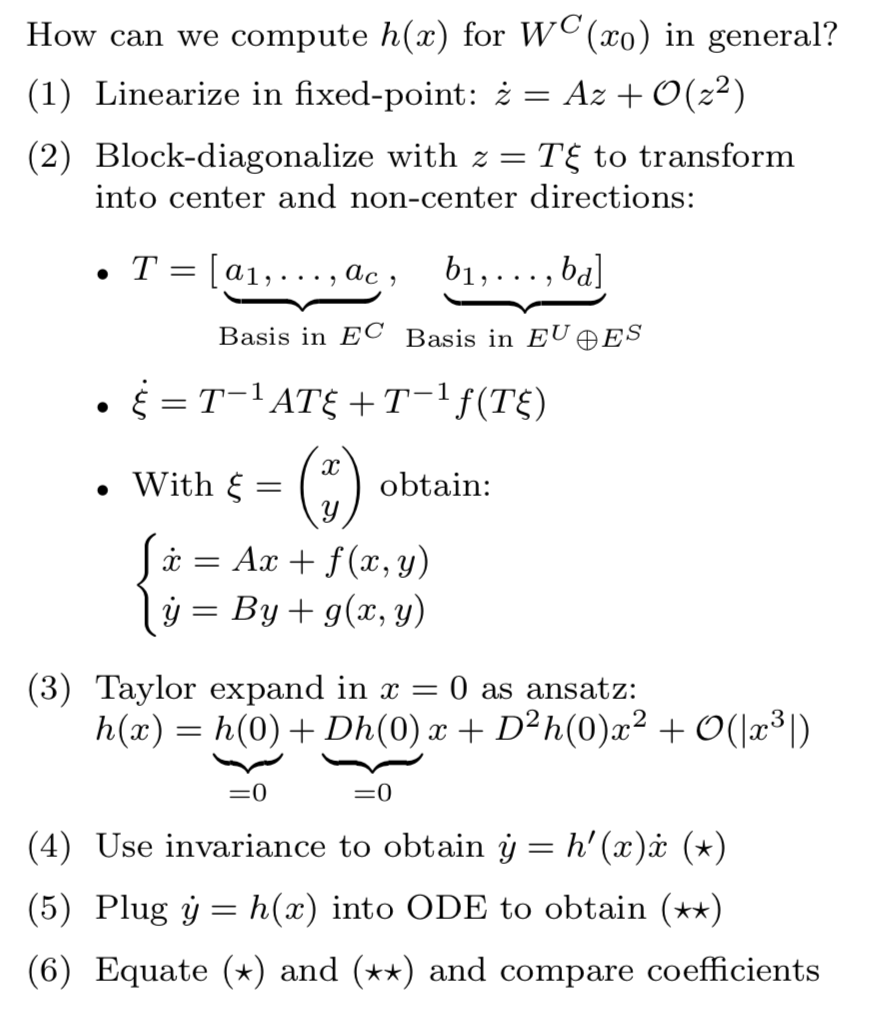
\includegraphics[scale=0.5]{computeWc.png}[h!]



\newpage
\section{Tricks of the nonlinear dynamic trade}

\subsection{Commonly used tricks}
\begin{itemize}
    \item Roots of quadratic polynomial: 
$$x=\frac{-b\pm\sqrt{b^2-4ac}}{2a}$$
    \item While doing a near identity transform: $\frac{1}{1+z}=1-z + )(z^2)$
    \item \textbf{Taylor series}: $$\sum_{n=0} ^ {\infty} \frac {f^{(n)}(a)}{n!} (x-a)^{n}$$
    \item Taking full derivative of a functional:
$$\frac{dL}{dt}
= \frac{\partial L}{\partial t} + \sum_{i=1}^n \frac{\partial L}{\partial x_i}\frac{dx_i}{dt}$$
    \item \textbf{Some trig identities:}
    $$\sin(\alpha \pm \beta) = \sin \alpha \cos \beta \pm \cos \alpha \sin \beta$$
    $$\cos(\alpha \pm \beta) = \cos \alpha \cos \beta \mp \sin \alpha \sin \beta$$
    \textbf{Power reducing identities:}
    $$\sin^2\theta = \frac{1 - \cos (2\theta)}{2}$$
    $$\cos^2\theta = \frac{1 + \cos (2\theta)}{2}$$
    $$\sin^2\theta \cos^2\theta = \frac{1 - \cos (4\theta)}{8}$$
    $$\sin^3\theta = \frac{3 \sin\theta - \sin (3\theta)}{4}$$
    $$\cos^3\theta = \frac{3 \cos\theta + \cos (3\theta)}{4}$$
    $$\sin^3\theta \cos^3\theta = \frac{3\sin (2\theta) - \sin (6\theta)}{32}$$
    $$\sin^4\theta = \frac{3 - 4 \cos (2\theta) + \cos (4\theta)}{8}$$
    $$\cos^4\theta = \frac{3 + 4 \cos (2\theta) + \cos (4\theta)}{8}$$
    $$\sin^4\theta \cos^4\theta = \frac{3-4\cos (4\theta) + \cos (8\theta)}{128}$$
    \textbf{Product-to-sum identities:}
    $$2\cos \theta \cos \varphi = {{\cos(\theta - \varphi) + \cos(\theta + \varphi)}}$$
    $$2\sin \theta \sin \varphi = {{\cos(\theta - \varphi) - \cos(\theta + \varphi)}}$$
    $$2\sin \theta \cos \varphi = {{\sin(\theta + \varphi) + \sin(\theta - \varphi)} }$$
    $$2\cos \theta \sin \varphi = {{\sin(\theta + \varphi) - \sin(\theta - \varphi)} }$$
   \item Linear algebra: 
\quad A =
\begin{pmatrix}
    a & b\\
    c & d
\end{pmatrix}
\begin{enumerate}
    \item \textbf{Trace}: $\operatorname{tr}(A) = \sum_{i=1}^{3} a_{ii}=a+d$
    \item \textbf{Inverse:} 
    $B^{-1} = \frac{1}{ad-cb}$
    \begin{pmatrix}
    d & -b\\
    -c & a
\end{pmatrix}
\end{enumerate}

\end{itemize}

\section{Useful definitions from lecture}
\begin{itemize}
    \item \textbf{Algebraic multiplicity of an eigenvalue} = number of times lambda appears as a root of the characteristic polynomial
    \item \textbf{Geometric multiplicity} = dimension of the eigenspace for the eigenvalue lambda. The eigenspace for lambda is given by:
    $$N(A-\lambda I)$$
    $$\text{dim(original matrix)=rank+nullity}$$
    That's how he gets that the geometric multiplicity is 1! Also note that:
    $$\text{geometric multiplicity}\leq \text{algebraic multiplicity}$$
\end{itemize}

\subsection{ODEs and PDEs}
\subsubsection{Separable differentiable equations}
You separate the $y$ and $dy$ from the $x$ and $dx$. Then you can integrate both sides. \textbf{It is usually the first thing you try!}
\begin{align*}
    &\frac{dy}{dx} = \frac{-x}{ye^{x^2}}
    \iff y\cdot dy=-xe^{x^2}dx\\
    & \int_{-\infty}^{+\infty} y\cdot dy = \int_{-\infty}^{+\infty}-xe^{x^2}dx \\
    & \iff \frac{y^2}{2} + C_1 = \frac{1}{2}e^{-x^2}+C_2
\end{align*}
This last formulation is called \textbf{the implicit form}  . And then you solve for y.

\subsubsection{Exact equations}
Consider: $$M(x,y) + N(x,y)\frac{dy}{dx} = 0$$\\
If: $$\frac{\partial M}{\partial y} = \frac{\partial N}{\partial x}$$
Then you have an \textbf{exact differential equation} and there is a $\Psi$ such that:
$$\frac{d\Psi(x,y)}{dx}=0$$
and 
$$\Psi(x,y)=C, \quad \frac{\partial \Psi}{\partial x}=M, \quad
\frac{\partial \Psi}{\partial y}=N$$

\href{https://www.khanacademy.org/math/differential-equations/first-order-differential-equations/modal/v/exact-equations-example-2}{Example from Khan Academy} to know how to solve this kind of problem.

\subsection{Second order differential equations}
\subsubsection{Linear}
$$a(x)y''+b(x)y'+c(x)y=d(x)$$

\subsubsection{Homogeneous 2nd order differential equations}
$$Ay''+By'+Cy=0$$
\begin{itemize}
    \item \textbf{Superposition applies:} If $g(x)$ and $h(x)$ are both solutions, then $a\cdotg(x)+b\cdoth(x)$ is also a solution.
    \item \textbf{Characteristic equation}: $Ar^2+Br+C=d(x)$
    \item \textbf{Most general solution:} $y(x)=C_1e^{r_1x}+C_2e^{r_2x}$
    \item \textbf{Solution for complex roots}: $r=\lambda \pm \mu i$
    $$y(x)=C_1e^{(\lambda + \mu i)x}+C_2e^{(\lambda - \mu i)x}$$
$$y(x)= e^{\lambda x}(C_1e^{\mu xi}+C_2e^{-\mu xi})$$
Given that: $e^{ix}=cosx+isinx$\\
We get:
$$y=e^{\lambda x}(C_3cos(\mu x)+C_4sin(\mu x))$$
    \item \textbf{Repeated roots:} similar to what you had before but now you need to add an x in front!
$$y(x)=C_1\cdot x \cdot e^{r_1x}+C_2e^{r_2x}$$
\end{itemize}

\subsubsection{Non-homogeneous ODE}
$$Ay''+By'+Cy=g(x)$$
You define:
\begin{itemize}
    \item \textbf{Homogeneous solution}
    \item \textbf{Particular solution}.
You can use the \textbf{method of undetermined coefficients}.
\end{itemize}
And you find a  \\
If $g(x)$ is of the form:
\begin{align}
    k e^{a x} \quad \rightarrow \quad C e^{a x}\\
    k x^n, n = 0, 1, 2 \ldots \quad \rightarrow \quad  \sum_{i=0}^n K_i x^i\\
    k \cos(a x) \text{ or } k \sin(a x) \quad \rightarrow \quad  K \cos(a x) + M \sin(a x)\\
    k e^{a x} \cos(b x) \text{ or } ke^{a x} \sin(b x) \quad \rightarrow \quad e^{a x} (K \cos(b x) + M \sin(b x))
    % \left(\sum_{i=0}^n k_i x^i\right) \cos(b x) \text{ or }\ \left(\sum_{i=0}^n k_i x^i\right) \sin(b x) \quad \rightarrow \quad \left(\sum_{i=0}^n Q_i x^i\right) \cos(b x) + \left(\sum_{i=0}^n R_i x^i\right) \sin(b x)\\
    % \left(\sum_{i=0}^n k_i x^i\right) e^{a x} \cos(b x) \text{ or } \left(\sum_{i=0}^n k_i x^i\right) e^{a x} \sin(b x) \quad \rightarrow \quad e^{a x} \left(\left(\sum_{i=0}^n Q_i x^i\right) \cos(b x) + \left(\sum_{i=0}^n R_i x^i\right) \sin(b x)\right) 
\end{align}


\end{multicols}

\end{document}
